\begin{figure*}[tp]
\centering
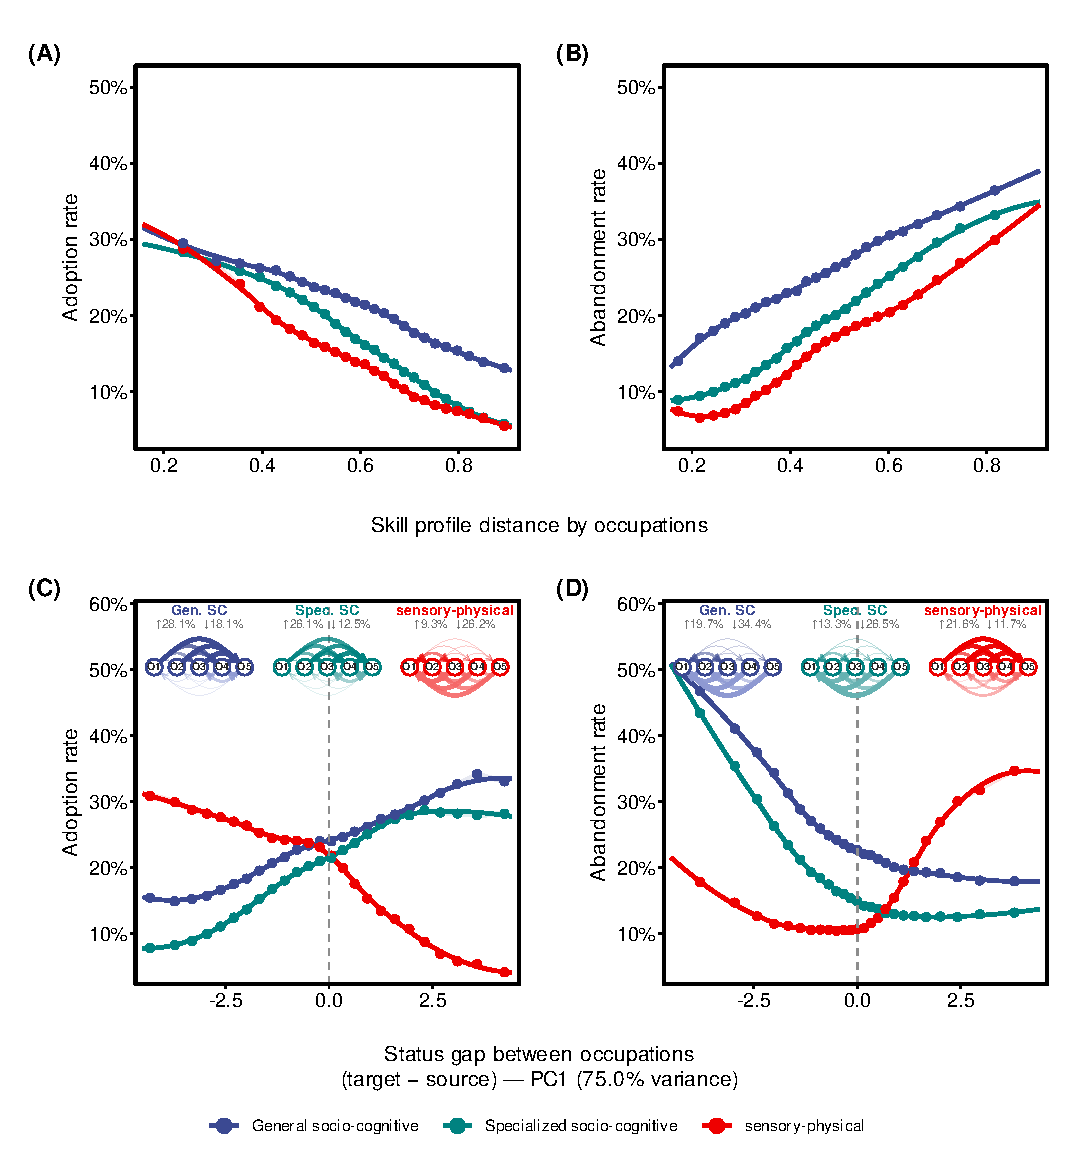
\includegraphics[width=.88\textwidth]{figures/fig1_full_networks.pdf}
\caption{%
\textbf{Skill adoption and abandonment rates as a function of skill-profile distance and occupational status gap.}
Colors distinguish three skill types throughout: \textcolor[HTML]{3B4992}{\textbf{general socio-cognitive}}, \textcolor[HTML]{008280}{\textbf{specialized socio-cognitive}}, and \textcolor[HTML]{EE0000}{\textbf{sensory-physical}}. In all panels, solid dots represent binned mean rates across 25 equal-frequency bins, shaded ribbons show 95\% bootstrap confidence intervals, and solid curves display LOESS-smoothed trends.
\textbf{(A, B)}~Adoption (A) and abandonment (B) rates plotted against the cosine distance between the skill-specialization profiles of the source and target occupations (higher values = less related).
\textbf{(C, D)}~Adoption (C) and abandonment (D) rates plotted against the composite PC1 status gap (target minus source; see Methods). Negative values indicate the target ranks below the source (downward gap), while positive values indicate the target ranks above (upward gap). The dashed vertical line marks zero.
\textbf{Insets:} The network diagrams in panels C and D show directional flow rates aggregated to status quintiles (Q1 = lowest, Q5 = highest). Each arc connects a source quintile to a destination quintile, with arc width and opacity proportional to the normalized directional flow rate within each skill class. Darker, right-pointing arcs indicate upward flows; lighter, left-pointing arcs indicate downward flows. Subtitle percentages report the overall mean upward ($\uparrow$) and downward ($\downarrow$) cross-quintile rates computed over the respective risk sets. O*NET, 2015--2024.
}
\label{fig:flows_gradients}
\end{figure*}
